

\subsection{Definition}

A \wddef{contact structure} on an oriented 3-manifold $M$ is a certain kind of
plane filed over $M$. More precisely it is a rank 2 sub-bundle $\xi \subset TM$,
given locally by the kernel of a one-form $\alpha$ (ie. for all $x\in M$,
$\exists U \subset M$, such that $\xi_x = \ker(\alpha_x)$ for all $x\in U$)
satisfying 
\begin{equation} 
\label{eq:alpha_non_zero}
\alpha \wedge \d \alpha \ne 0. \quad \text{(ie. everywhere non-zero.)}
\end{equation}

We will also require that $\alpha \wedge \d \alpha$ agrees with the orientation
orientation of $M$.
Intuitively condition \pref{eq:alpha_non_zero}, require the planes to be
twisting, see figure \pref{fig:stand_contact}. Because of this twisting, there
can not be a surface in $S \subset M$, such that $\xi|S = TS$. 
A \wddef{contact manifold} is a pair $(M,\xi)$, where $M$ is an oriented
3-manifold and $\xi$ is a contact structure on $M$.

\begin{figure}
\centering
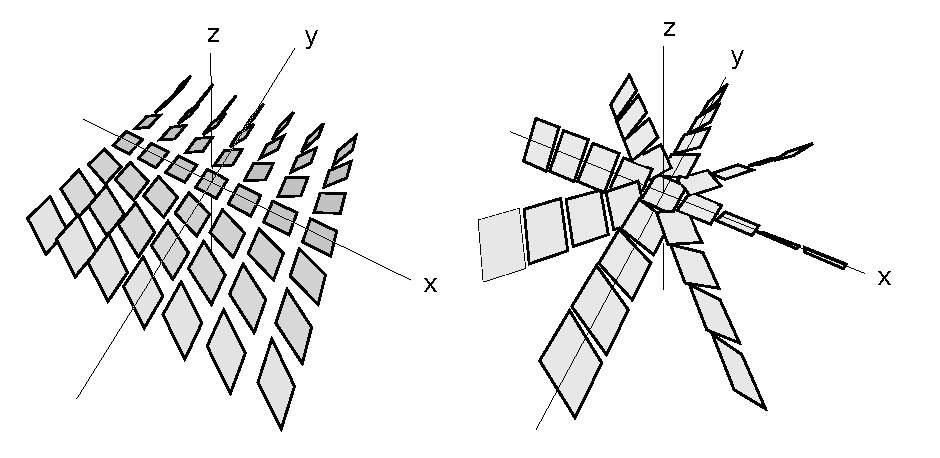
\includegraphics[width=.4\textwidth]{figs/stand_contact.pdf}
\caption{Contact structure $\xi_{std}$ (left) and $\xi_{sym}$ (right). }
\label{fig:stand_contact}
\end{figure}

\subsection{Examples}

\begin{exmp}
Consider $M = \R^3$, with Cartesian coordinates $(x,y,z)$. Let $\alpha = \d z -
y \d x$, then $\alpha \wedge \d \alpha = \d x \wedge \d y \wedge \d z \ne 0$.
Define 
\[ \xi_{std} := \ker{\alpha} = \spann\qty{ \dd{y}, \dd{x} + y \dd{z} }. \]
$\xi_{std}$ is called the standard contact structure on $\R^3$. See fig
\pref{fig:stand_contact}.
\end{exmp} 
There are a couple key features of this plane filed. 
Note that restricted to a plane parallel with the $xz$-plane all the planes are
parallel, or sad in a different way the pane filed is invariant under
translations orthogonal to the $y$ direction. In particular the planes along the
$xz$-plane are all horizontal, that is parallel with the $xy$-plane. On the
other hand, when moving along the $y$-axis the planes twist in a left hand
manner. Twisting a total of $90^\circ$ going from the origin "to infinity" in
the $y$-direction. 

\begin{exmp}
Again let $M = \R^3$ and let $\alpha = \d z + x\d y - y \d x$ ( or $\alpha = \d
z + r^2 \d \theta$ in cylindrical coordinates.) Then $\alpha \wedge \d \alpha =
2 \d x \wedge \d y \wedge \d z \ne 0$, so $\alpha$ defines a contact structure.
Define 
\[  \xi_{sym} := \ker\alpha = \spann\qty{ \dd{r}, \dd \theta - r^2 \dd{z} }. \]
This is the symmetric version of $\xi_{std}$.
\end{exmp}


%  
% = \spann{ (\dd x)^2 +  }

Here the planes are invariant under vertical translations (along the $z$-axis)
and rotation about the $z$-axis. 

\begin{defn}
Let $M$ and $N$, be two oriented 3-manifolds and suppose $\xi_M$ and $\xi_N$ are
are contact structures on $M$ and $N$ respectively. 
A diffeomorphism $f: M \to N$ is called a \wddef{contactomorphism}, if $f_*$ maps
$\xi_M$ to $\xi_N$. 

If such a contactomorphism exist $\xi_M$ and $\xi_N$ are sad to be
\wddef{contactomorphic}.
\end{defn}


The contact structures $\xi_{std}$ and $\xi_{sym}$ are contactomorphic, so in
a way they are the same structure. 
%
%Let $f(x,y,z) = (x, y, z - x^2y )$
%
% Df = 
%    1  0 0
%    0  1 0
% -2xy -x^2 1
%
% $ f^* \alpha (dx, dy, dz) = \alpha \circ f_* (  )
%
Also suppose we defined $\xi_{std}$ with
the opposite sign (ie. $\alpha = \d z + y\d x$), then the planes would instead
twist in a right handed manner, when moving in the $y$ direction. Then this
structure would be contactomorphic to $\xi_{std}$, by the diffeomorphism mapping
$y$ to $-y$.

\begin{exmp}
Let $M=\R^3$ and $\alpha = \cos r \d z + r \sin r \d \theta$ and define the
contact structure $\xi_{ot} = \ker \alpha$. See fig \pref{fig:overtwisted}
\end{exmp}

\begin{figure}
\centering
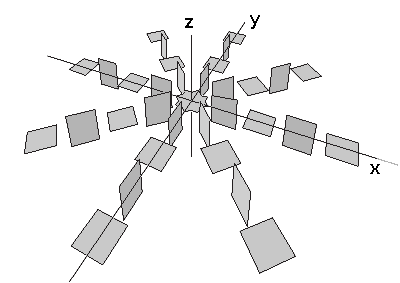
\includegraphics[width=.4\textwidth]{figs/overtwisted.pdf}
\caption{The overtwisted contact structure $\xi_{ot}$.}
\label{fig:overtwisted}
\end{figure}

Note how this structure in a way is very similar to $\xi_{sym}$, except that
when moving along a ray perpendicular to the $z$-axis, the twisting is much
quicker. So in instead of rotating a total of $90^\circ$ when going to infinity,
the planes are already twisted $90^\circ$ when getting to a radius of $\pi/2$ and
rotates an infinite number of times when going to infinity.

\begin{defn}
Suppose $\xi$ defines a contact structure on $M$. Then, we say $\xi$ is
\wddef{overtwisted}, if there exist an immersion $u : D(0,1) \to M$, where
$D(0,1) = \{ (x,y) \in \R^2 \q| x^2+y^2 \le 1 \}$ is the unit disk, such that
\[ \xi|_{\partial D} = TD|_{\partial D}. \]
(ie. $\xi$ is tangent to $D$ along the border of $D$.) Such a disk immersion is
called an \wddef{overtwisted disk}.

If $\xi$ is not overtwisted we say $\xi$ is \wddef{tight}.
\end{defn}

Clearly $\xi_{ot}$ is overtwisted since $D = \{ (r,\theta, z) \q| z = 0, 0 \le
r \le 1\}$ is an overtwisted disk. On the other hand $\xi_{std}$ and $\xi_{sym}$
are tight. It turns out that tight contact structures are more interesting then
the overtwisted ones, see \cite{Eliashberg1989}. In this paper we will mainly
concentrate on $(\R^3, \xi_{std})$. However, we will mention one other example.   

\begin{exmp}
Let $M=S^3$ considered as the unit sphere in $\R^4$ (with Cartesian coordinates
$(x_1,y_1,x_2,y_2)$), and let 
\[ \alpha = i^*( x_1 \d y_1 - y_1 \d x_1 + x_2 \d y_2 - y_2 \d x_2 ), \]
where $i: S^3 \R^4$ is the inclusion map. One may check that $\alpha \wedge \d
\alpha \ne 0$, and define $\xi = \ker \alpha$.
\end{exmp}

By removing one point $p$ from $S^3$, the contact structure $\xi$ on $S^3 \setminus
\{p\}$ is
contactomorphic to $\xi_{sym}$ (and thus $\xi_{std}$) on $\R^3$. 

In fact, if we associate $\R^4$ with $\C^2$, we can construct this contact
structure from the complex structure on $C^2$. Let $J$ denote complex
multiplication in $\C^2$, ie. $J x_i = y_i$ and $J y_i = x_i$ for $i=1,2$. This
complex structure includes a complex structure on the tangent space $J
\dd{x_i} = \dd{y_i}$ and $J\dd{y_i} = \dd{x}$.

\begin{clame}
Then $\xi$ is the complex tangents of $S^3$. ie.
\[  \xi = TS^3 \cap J (TS^3), \]
that is the tangent space closed under complex multiplication. 
\end{clame}

\begin{proof}
Let $f:R^4 \to R^4$, defined by $f(x_1,y_1,x_2,y_2) = x_1^2+y_1^2+x_2^2+y_2^2$,
then $S^3 = f^{-1}(1)$. Then the tangent space of $S^3$ at $(x_1,y_1,x_2,y_2)$
\[ T_{(x_1,y_1,x_2,y_2)}S^3 = \ker{ \d f_{(x_1,y_1,x_2,y_2)} },   \]
and 
\[ J (T_{(x_1,y_1,x_2,y_2)}S^3) = \ker{ \d f_{(x_1,y_1,x_2,y_2)} \circ J}. \]
Since 
\[ \d f_{(x_1,y_1,x_2,y_2)} \circ J = 2 x_1 \d y_1 - 2 y_1 \d x_1 + 2 x_2 \d y_2 - 2 y_2 \d x_2 \]
So $\alpha = (\d f \circ J)|_S^3$, which proves the clime.
\end{proof}


% \subsection{Relation to simplistic geometry}

